\documentclass{beamer}

\mode<presentation> {
\usetheme{Madrid}
}

\beamertemplatenavigationsymbolsempty

% pacman.sty does not allow numbering pages properly with backup/appendix slides
% \usepackage{pacman} % Allows you to be the best presentator ever :D

\usepackage{graphicx} % Allows to include figures
% \usepackage{booktabs} % Allows the use of \toprule, \midrule and \bottomrule in tables
% \usepackage[utf8]{inputenc}
% \usepackage{float}
% \usepackage{mathtools}
% \usepackage{xcolor}
% \usepackage{bm}
% \usepackage{scalerel}
% \usepackage{setspace}
% \usepackage{appendixnumberbeamer} % add \appendix

% \usepackage{amsmath}
% \usepackage{amssymb}
\usepackage{mathtools, nccmath}
% \usepackage[mathscr]{euscript}  % euler script font
% \usepackage{cleveref}
% \usepackage{enumitem}

\usepackage{algorithm}
\usepackage[noend]{algpseudocode}

\DeclareMathOperator{\Var}{Var}
\DeclareMathOperator{\modexp}{mod\_exp}
\DeclareMathOperator{\decryptiontime}{decryption\_time}
\DeclareMathOperator{\extrareduction}{extra\ reduction}

%---------------------------------------------------------------------------------------
%	TITLE PAGE
%---------------------------------------------------------------------------------------

\title[DSP - 2021/22 - Lorenzo Palloni]{Timing Attacks against RSA}
\subtitle{(DSP \footnote{Data Security and Privacy} - Project implementation)}
\author{Lorenzo Palloni}
\institute[]{
  University of Florence\\
  \medskip
  \textit{lorenzo.palloni@stud.unifi.it}
}
\date{\today}

\begin{document}

\begin{frame}
\titlepage % Print the title page as the first slide
\end{frame}

%---------------------------------------------------------------------------------------
%	PRESENTATION SLIDES
%---------------------------------------------------------------------------------------
%   TABLE OF CONTENTES
%---------------------------------------------------------------------------------------
%\begin{frame}
%\tableofcontents
%\end{frame}
%---------------------------------------------------------------------------------------
% - kocher_main.py
%   - Implementation of Kocher's timing attack using TimingAttackModule.py provided by the professor.
%   - It uses dynamic number of ciphertexts each iteration (i.e. for each bit to be guessed)
% - kocher_output.txt
%   - displays the output of a successful kocher_main.py run
% - old-openssl_timing_attack.py
%   - old stuff
% - brumley_and_boneh_main.py
%
% - optimize_rabin_sequence_generation.py
%   - Rabin test implementation (that can be found in utilities.py) was too slow.
%   - This script helped to
% - prime_numbers_lower_than_2000.txt
% - stats.dump
% - test_utilities.py
% - TimingAttackModule.py
% - utilities.py
%---------------------------------------------------------------------------------------
\begin{frame}
\frametitle{Introduction}

\begin{itemize}

  \item \emph{What are we going to talk about?}
  \begin{itemize}
    \item Some implementations related to the exam project.
  \end{itemize}
  \item \emph{What is the project about?}
  \begin{itemize}
    \item An overview of two major timing attacks:
    \begin{itemize}
      \item[$\rightarrow$] Kocher's timing attack (1996) \cite{bib:kocher};
      \item[$\rightarrow$] Brumley and Boneh's timing attack (2005) \cite{bib:openssl}.
    \end{itemize}
  \end{itemize}
\end{itemize}

\end{frame}
%---------------------------------------------------------------------------------------
\begin{frame}
\frametitle{Main source files}
% - kocher_main.py
%   - Implementation of Kocher's timing attack using TimingAttackModule.py provided by the professor.
%   - It uses dynamic number of ciphertexts each iteration (i.e. for each bit to be guessed)
% - kocher_output.txt
%   - displays the output of a successful kocher_main.py run
% - old-openssl_timing_attack.py
%   - old stuff
% - brumley_and_boneh_main.py
% - optimize_rabin_sequence_generation.py
%   - Rabin test implementation (that can be found in utilities.py) was too slow.
% - prime_numbers_lower_than_2000.txt
% - stats.dump
% - test_utilities.py
% - TimingAttackModule.py
% - utilities.py

\begin{itemize}
  \item kocher\_main.py
  \begin{itemize}
    \item[$\rightarrow$] Kocher's timing attack;
  \end{itemize}
  \item brumley\_and\_boneh\_main.py
  \begin{itemize}
    \item[$\rightarrow$] Brumley and Boneh's timing attack;
  \end{itemize}
  \item utilities.py
  \begin{itemize}
    \item[$\rightarrow$] Random prime number generator from scratch;
    \item[$\rightarrow$] RSA (that comes easily with the previous point);
    \item[$\rightarrow$] other utility functions.
  \end{itemize}
\end{itemize}

\end{frame}
%---------------------------------------------------------------------------------------
\begin{frame}
\frametitle{utilities.py}
\setbeamertemplate{enumerate items}[default]

{\small
  \begin{enumerate}
    \item gen\_rsa\_factors(half\_k: int = 8, seed: int = None) $\rightarrow$ Tuple[int, int];
    {\onslide<2->
      \item gen\_prime(low: int, high: int, seed: int = None, tries: int = 3) $\rightarrow$ int;
    }
    {\onslide<3->
      \item gen\_odd(low: int, high: int, seed: int = None) $\rightarrow$ int;
    }
    {\onslide<4->
      \item is\_probably\_prime(guess: int, tries: int = 4) $\rightarrow$\ bool;
    }
    {\onslide<5->
    \item rabin\_test(n: int, x: int = None, verbose: bool = False) $\rightarrow$\ bool;
    }
    {\onslide<6->
    \item gen\_rabin\_sequence(n: int, x: int, m: int, r: int) $\rightarrow$\ List[int];
    }
    {\onslide<7->
    \item get\_m\_and\_r(n: int) $\rightarrow$\ Tuple[int, int];
    }
    {\onslide<8->
    \item check\_quadratic\_residuals(n: int, seq: List[int]) $\rightarrow$\ bool;
    }
    {\onslide<9->
    \item mod\_exp(a: int, m: int, n: int) $\rightarrow$\ int;
    }
    {\onslide<10->
    \item binarize(a: int) $\rightarrow$\ List[int];
    }
    {\onslide<11->
    \item binarize\_inverse(a: List[int]) $\rightarrow$\ int;
    }
    {\onslide<12->
      \item gcd(a: int, b: int) $\rightarrow$\ Tuple[int, int].
    }
  \end{enumerate}
}

\end{frame}
%---------------------------------------------------------------------------------------
\begin{frame}
\frametitle{kocher\_main.py}

\begin{itemize}
  \item Kocher's timing attack;
  \item devices simulated with TimingAttackModule.py \footnote{Professor Michele Boreale provided it.};
  \item dynamic number of ciphertexts for each iteration (i.e. for each bit).
\end{itemize}

Output example:

{\onslide<2->
  \center
  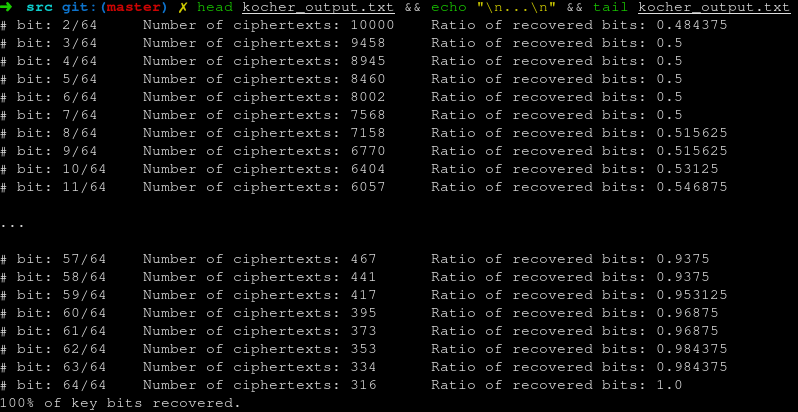
\includegraphics[width=0.75\textwidth]{figures/kocher_output_example}
}

\end{frame}
%---------------------------------------------------------------------------------------
\begin{frame}
\frametitle{brumley\_and\_boneh\_main.py}

\begin{itemize}
  \item Brumley and Boneh's timing attack;
  \item Two classes implemented:
  \begin{itemize}
    \item class $Device$
    \item class $Attacker$
  \end{itemize}
\end{itemize}

\end{frame}
%---------------------------------------------------------------------------------------
\begin{frame}
\frametitle{brumley\_and\_boneh\_main.py}

\begin{itemize}
  \item class $Device$
  \begin{itemize}
    {\onslide<2->
      \item \_\_init\_\_(
      \begin{itemize}
        \item[] self,
        \item[] num\_bits: int = 16,
        \item[] seed: int = None,
        \item[] blinding: bool = False
      \end{itemize}
      \item[] );
    }
    {\onslide<3->
      \item gen\_montgomery\_coefficient(self) $\rightarrow$\ int;
    }
    {\onslide<4->
      \item get\_modulus(self) $\rightarrow$\ int;
    }
    {\onslide<5->
      \item run(self, u: int) $\rightarrow$\ float;
    }
    {\onslide<6->
      \item \_decryption(self, u: int) $\rightarrow$\ float;
    }
    {\onslide<7->
      \item \_get\_factors(self) $\rightarrow$\ Tuple[int, int];
    }
  \end{itemize}
\end{itemize}

\end{frame}
%---------------------------------------------------------------------------------------
\begin{frame}
\frametitle{brumley\_and\_boneh\_main.py}

\begin{itemize}
  \item class $Attacker$
  \begin{itemize}
    {\onslide<2->
      \item \_\_init\_\_(
      \begin{itemize}
        \item[] self,
        \item[] device: Device,
        \item[] num\_bits\_per\_factor: int = None,
        \item[] modulus: int = None,
        \item[] montgomery\_coefficient: int = None,
      \end{itemize}
      \item[] );
    }
    {\onslide<3->
      \item guess(self, threshold: float = 4e-4) $\rightarrow$\ int;
    }
    {\onslide<4->
      \item plot\_last\_guess(self, savefig\_path=None, figsize=None).
    }
  \end{itemize}
\end{itemize}

\end{frame}
%---------------------------------------------------------------------------------------
\begin{frame}
\frametitle{brumley\_and\_boneh\_main.py}
\setbeamertemplate{enumerate items}[default]

{\scriptsize
\begin{block}{Code snippet}
  \begin{enumerate}
      \item device = Device(num\_bits=64, seed=42, blinding=False)
      \item attacker = Attacker(device)
      \item g = attacker.guess()
      \item attacker.plot\_last\_guess()
  \end{enumerate}
\end{block}
}

\center
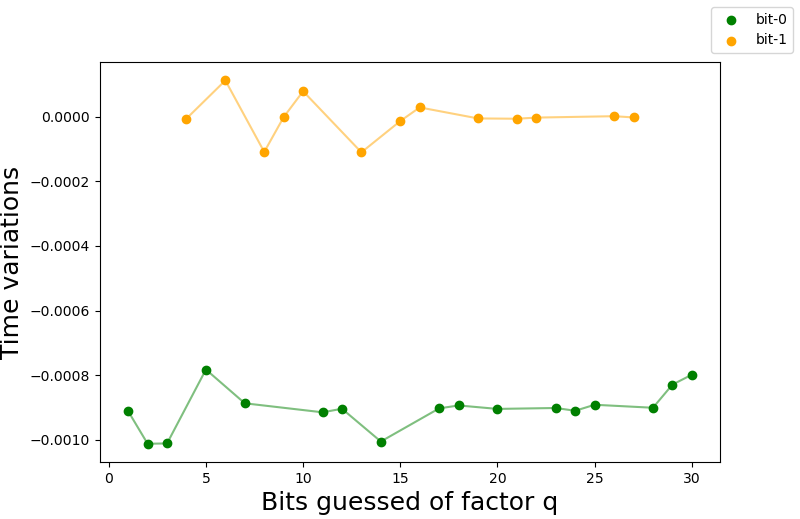
\includegraphics[width=0.65\textwidth]{figures/brumley_and_boneh_output_example}

\end{frame}
%---------------------------------------------------------------------------------------
\begin{frame}
\frametitle{brumley\_and\_boneh\_main.py}

\begin{itemize}
  \item \emph{What is in the guess \textbf{g} of this example?}
  \begin{itemize}
    \item[$\rightarrow$] $2330302001$
  \end{itemize}
  \item \emph{...and the actual factor \textbf{q}?}
  \begin{itemize}
    \item[$\rightarrow$] $2330302003$
  \end{itemize}
  \item \emph{How does the guess \textbf{binarize(g)} look like?}
  \begin{itemize}
    \item[$\rightarrow$] $[1, 0, 0, 1, 0, \dots, 1, 0, 0, \mathbf{0, 1}]$
  \end{itemize}
  \item \emph{...and what about \textbf{binarize(q)}?}
  \begin{itemize}
    \item[$\rightarrow$] $[1, 0, 0, 1, 0, \dots, 1, 0, 0, \mathbf{1, 1}]$
  \end{itemize}
\end{itemize}

\end{frame}
%---------------------------------------------------------------------------------------
\begin{frame}
\frametitle{brumley\_and\_boneh\_main.py}
\setbeamertemplate{enumerate items}[default]

{\scriptsize
\begin{block}{Code snippet}
  \begin{enumerate}
      \item device = Device(num\_bits=64, seed=42, blinding=\textbf{True})
      \item attacker = Attacker(device)
      \item g = attacker.guess()
      \item attacker.plot\_last\_guess()
  \end{enumerate}
\end{block}
}

\center
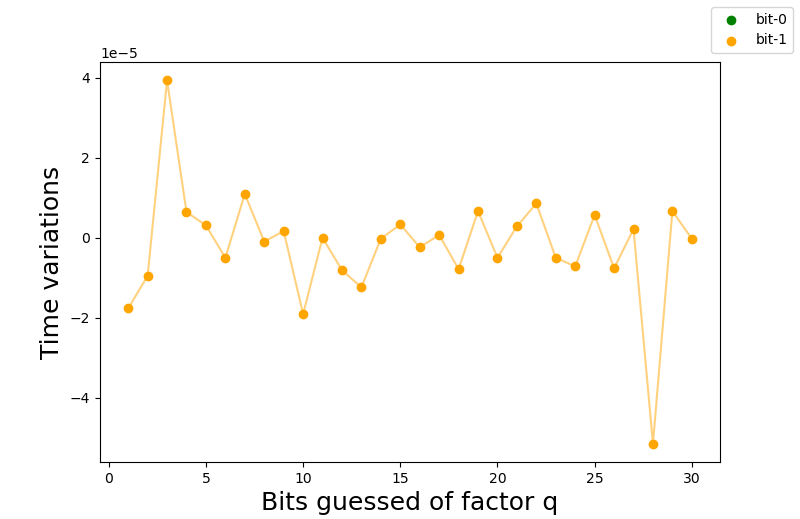
\includegraphics[width=0.65\textwidth]{figures/brumley_and_boneh_output_example_with_blinding}

\end{frame}
%---------------------------------------------------------------------------------------
\begin{frame}
\frametitle{brumley\_and\_boneh\_main.py / Device.\_decryption}
\setbeamertemplate{enumerate items}[default]

Device.\_decryption(self, u: int) $\rightarrow$ float:

\begin{enumerate}

% \item applies blinding if it is activated;
\item convert the input $u$ in its Montgomery form $\rightarrow g$;
\item initialize $t_q := 0$ and $t_p := 0$;
\item if $g < self.q$, then:
  \begin{itemize}
    \item $t_q = t_q + 1000$ (many Montgomery reductions);
    \item $t_q = t_q + 100$ (normal multiplication routine);
  \end{itemize}
\item[] otherwise ($g \ge self.q$):
  \begin{itemize}
    \item $t_q = t_q + 10$ (few Montgomery reductions);
    \item $t_q = t_q + 10$ (Karatsuba multiplication routine);
  \end{itemize}
\item repeat step 3. with $self.p$ (updating $t_p$);
\item $time.sleep(\frac{\mathcal{N}(t_q + t_p,\ 5)}{1e6})$.
\end{enumerate}

\end{frame}
%---------------------------------------------------------------------------------------
%---------------------------------------------------------------------------------------
%---------------------------------------------------------------------------------------
%---------------------------------------------------------------------------------------
%---------------------------------------------------------------------------------------
\begin{frame}[c,noframenumbering]

  \LARGE \emph{Do you have any questions?}

\end{frame}
%---------------------------------------------------------------------------------------
\begingroup
\footnotesize
\begin{frame}[noframenumbering]
\frametitle{References}
\begin{thebibliography}{99}

\bibitem{bib:kocher}{Kocher, P.C., 1996, August. Timing attacks on implementations of Diffie-Hellman, RSA, DSS, and other systems. In Annual International Cryptology Conference (pp. 104-113). Springer, Berlin, Heidelberg.}
\bibitem{bib:openssl}{Brumley, D. and Boneh, D., 2005. Remote timing attacks are practical. Computer Networks, 48(5), pp.701-716.}
% \bibitem{bib:boreale}{Boreale, M., 2003. Note per il corso di Sicurezza delle Reti.}
% \bibitem{bib:montgomery}{Montgomery, P.L., 1985. Modular multiplication without trial division. Mathematics of computation, 44(170), pp.519-521.}
% \bibitem{bib:sliding}{Menezes, A.J., Van Oorschot, P.C. and Vanstone, S.A., 2018. Handbook of applied cryptography. CRC press.}
% \bibitem{bib:schindler}{Schindler, W., 2000, August. A timing attack against RSA with the chinese remainder theorem. In International Workshop on Cryptographic Hardware and Embedded Systems (pp. 109-124). Springer, Berlin, Heidelberg.}
% \bibitem{bib:coppersmith}{Coppersmith, D., 1997. Small solutions to polynomial equations, and low exponent RSA vulnerabilities. Journal of cryptology, 10(4), pp.233-260.}

\end{thebibliography}
\end{frame}
\endgroup
%---------------------------------------------------------------------------------------

\end{document}

